\section{FamilySearch i la segona guerra mundial: La llista de Schindler}

    \paragraph{}
    Aquesta proposta pretén realitzar un estudi sobre un dels col·lectius que es va veure més afectat durant la segona guerra mundial, els jueus.

    Aquesta proposta de projecte ofereix a l'estudiant parcejar els cognoms coneguts d'aquelles persones que van formar la llista de Schindler i realitzar un estudi d'aquests cognoms sobre les dades de FamilySearch.

    El projecte pot intentar respondre preguntes com: Van disminuir en gran quantitat el nombre de registres amb els cognoms indicats? Van realitzar aquestes persones un procés d'emigració a diferents indrets del món? En quins moments es van començar a produir aquestes emigracions? Quina mena de documents han quedat enregistrats al respecte?

    La proposta que ens ocupa se'm va acudir quan vaig descobrir, en les fases prèvies del projecte, el certificat d'emigració de Wladyslaw Szpilman, també conegut, com el pianista de Varsòvia. La imatge~\ref{fig:thePianist} mostra el registre físic que pot ser trobat a FamilySearch.

    \begin{figure}[h]
        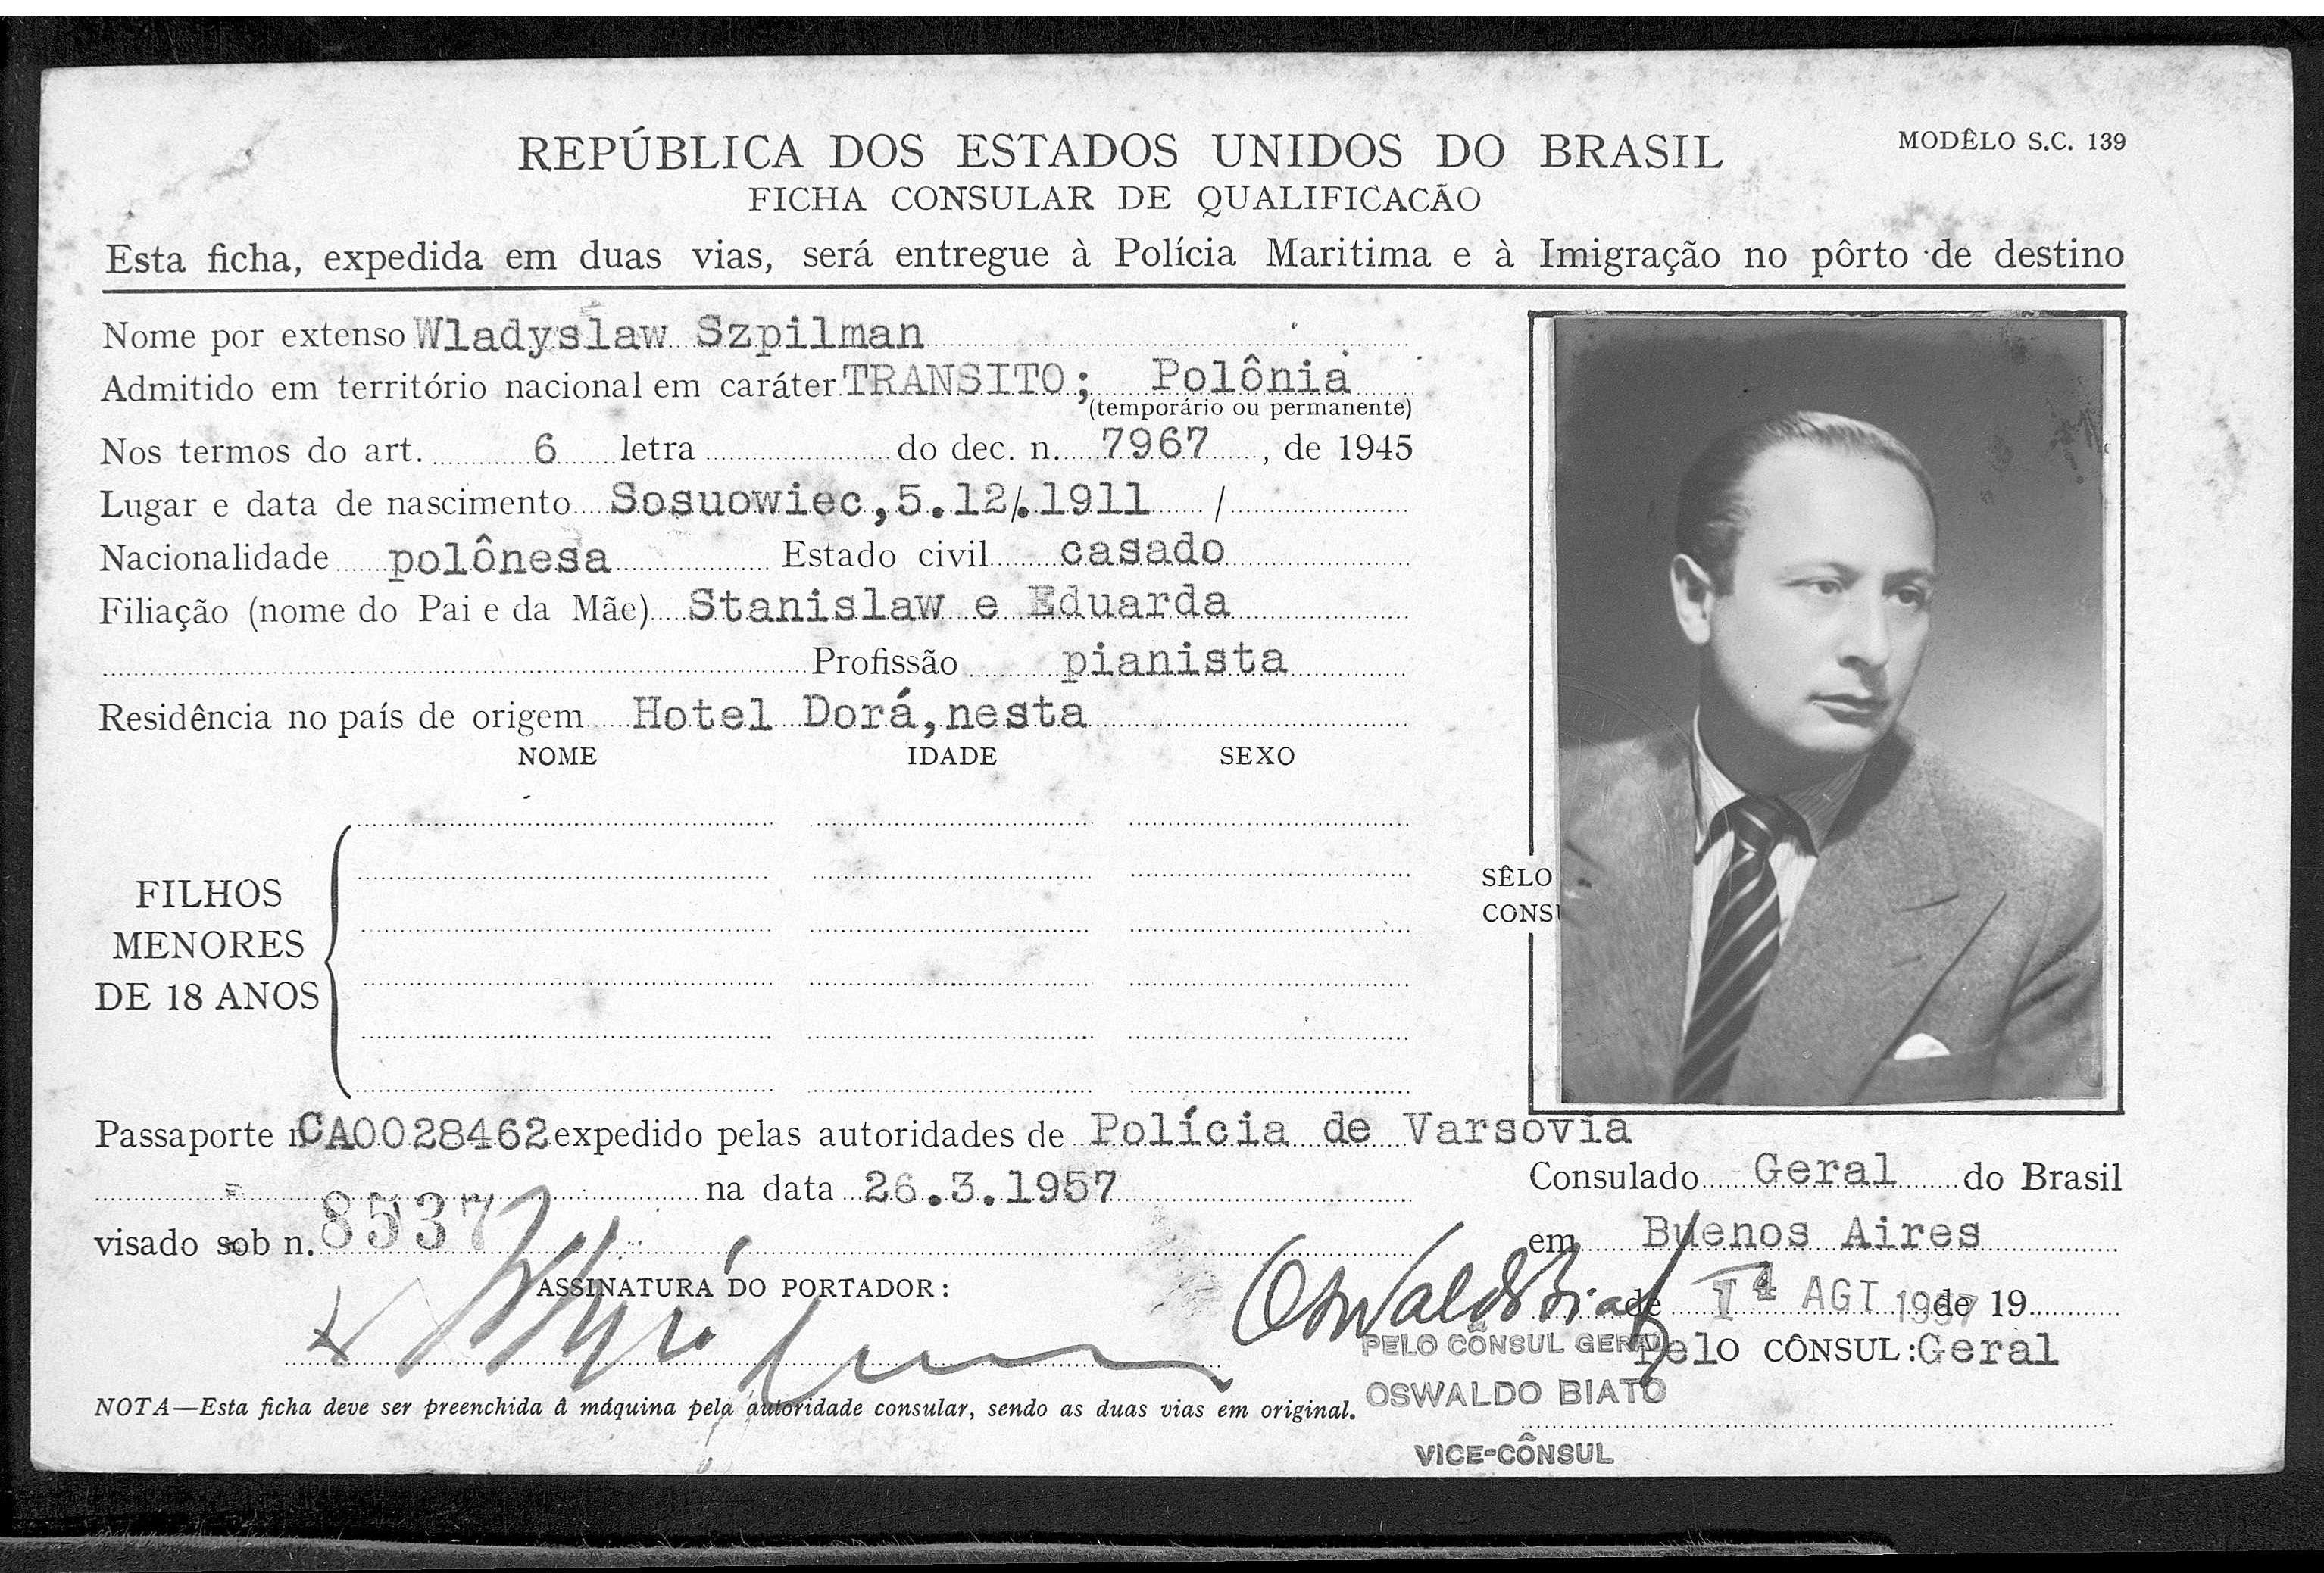
\includegraphics[width=\linewidth]{07/thePianist}
        \centering
        \caption{Registre d'emigració de \emph{Wladyslaw Szpilman}\label{fig:thePianist}}
    \end{figure}
